
\documentclass{acm_proc_article-sp}

\usepackage{amsmath}
\usepackage{verbatim}
\usepackage{textcomp}
\usepackage{graphicx}
\usepackage{subcaption}
\usepackage{url}


\begin{document}

\title{Difficult Handwritten Digit Classification \\
{\normalsize Code available at: \url{https://github.com/slflmm/Miniproject-3}}} 
\subtitle{COMP 598 -- Miniproject 3 -- Team X}

\numberofauthors{3} 
\author{
% 1st. author
\alignauthor 
Narges Aghakazemjourabbaf\\
	\affaddr{?}
\alignauthor
Stephanie Laflamme\\
	\affaddr{260376691}
% 2nd. author
\alignauthor Benjamin La Schiazza\\
	\affaddr{?}
% 3rd. author
}

\date{Oct15}



\maketitle
\begin{abstract}

\end{abstract}

\section{Introduction}% overview of approach

\section{Preprocessing}
The raw pixels are standardized. For each example $i$ in the training set, and each feature $j$, we replace it with its standardized value $$x'_{ij} = \cfrac{x_{ij} - \mu_{j}}{\sigma_{j}}.$$

These values for $\mu_j$ and $\sigma_j$ are used to apply the same transformation to the test set examples.

\section{Feature Design and Selection}
When appropriate for the learner, we consider three feature sets; raw pixels, PCA, and Gabor filter-based features.

\subsection{Pixels}
We use the post-standardization pixel information as a baseline feature set.This produces feature vectors of length 2304. 

\subsection{PCA}
Principal component analysis (PCA), developed by Pearson in the early 1900s\cite{Pearson}, converts a set of possibly correlated features into a linearly uncorrelated representation, with the resulting features ordered by variance. 

We use the implementation of PCA provided by the Scikit-learn library\cite{scikit-learn}, which uses singular value decomposition of the input data matrix.

As removing the least useful features made the results of our baseline classifier worse, we keep full dimensionality. However, we expect PCA features to produce better results given that they are linearly uncorrelated.

\subsection{Gabor}
Gabor filters are linear filters used for edge detection and are thought to be similar to the early stages of visual processing in humans. Indeed, their frequency and orientations correspond roughly to simple cells in the visual cortex of humans and other mammals; these cells can be modelled with Gabor functions.\cite{Jones}\cite{Marvcelja} As these filters are well-suited to image processing, we attempt to translate them into features.

Previous research has used the energy of the convolution between a Gabor filters and image (a measure of how strongly the filter responds to that image\cite{Grigorescu}) as a feature by summing its magnitudes in the image.\cite{Bau} This is equivalent to using the Frobenius norm of the convolved image as a feature. 

Using the Scikit-learn library\cite{scikit-learn}, we generate 16 Gabor filters with 4 equidistant $\theta$ values, $\sigma = \{1, 3\}$, and frequencies $= \{0.05, 0.25\}$. Figure \ref{fig:gabor} illustrates the effects of $\theta$, $\sigma$, and frequency with a sample of our filters. We form the feature vector of an image in the dataset by collecting the Frobenius norms of the image convolved with each filter. 

\begin{figure}[h]
	\centering
	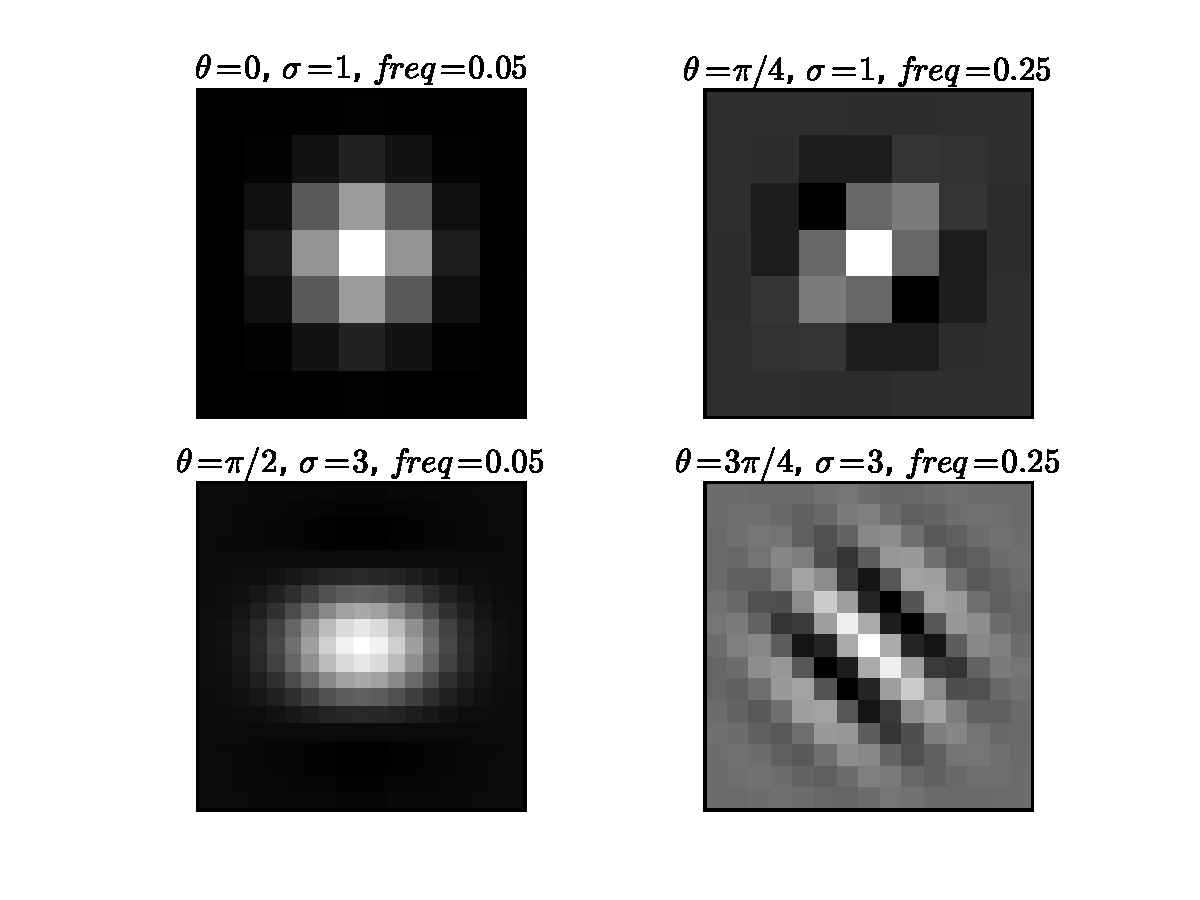
\includegraphics[width=\linewidth]{gabors}
  	\caption{Some Gabor filters}
  	\label{fig:gabor}
\end{figure}


\section{Algorithm Selection}% for each category
\subsection{Perceptron}
We implement a multiclass perceptron as a baseline classifier. Given $n$ examples with $m$ features each, the perceptron 

\subsection{Neural Network}

\subsection{Linear SVM}
Use Scikit-learn implementation \cite{scikit-learn}

\subsection{Convolutional Neural Network}
Origin of convnets \cite{Fukushima}. We can see it has good invariance to rotation and resistance to noise with the MNIST dataset. \cite{LeCun}

Problem of neural networks = overfitting. Regularization... (L1 + L2 norms). Dropout \cite{Hinton}
Dropout in fully-connected layers of a convolutional net \cite{Krizhevsky}
SGD with minibatches.
Momentum.


\section{Optimization} % if required
GPU for convolutional network -- Theano \cite{Theano}

\section{Parameter Selection Method}% model order, learning rate, etc
Preliminary manual search followed by either:

Gridsearch 

Random search \cite{Bergstra}

\section{Testing and Validation}%detailed analysis of results

\subsection{Perceptron}
In a primary step, we performed 5-fold cross-validation to compare raw pixels, PCA, and Gabor features using a fixed learning rate ($\alpha = 0.01$) and number of iterations (15). As shown in Table \ref{tab:perc-features}, PCA features were the most performant, with a validation accuracy of 26.282\%.
\begin{table}[h!]
  \centering
  \begin{tabular}{|c||c|c|c| }
    \hline
    {\bfseries Features} & Pixels & PCA & Gabor \\
    \hline
    {\bfseries Accuracy} & 25.794 & 26.282 & 10.398 \\
    \hline
  \end{tabular}
  \caption{Mean validation accuracy of perceptron using different features}
  \label{tab:perc-features}
\end{table}

Using (the best feature set), we performed 5-fold cross-validation over the learning rate $\alpha$ and the number of training iterations of the perceptron model. Figure \ref{fig:perc-gridsearch} shows the results of gridsearch with both parameters. The precise values of the best parameters found by the gridsearch cross-validation procedure were $\alpha = 0.0005$ with 25 training iterations, yielding a mean validation accuracy of 26.598\%.\footnote{Additional results showing training error vs validation error are shown in Appendix \ref{sec:additional-results}}
\begin{figure}[h!]
	\centering
	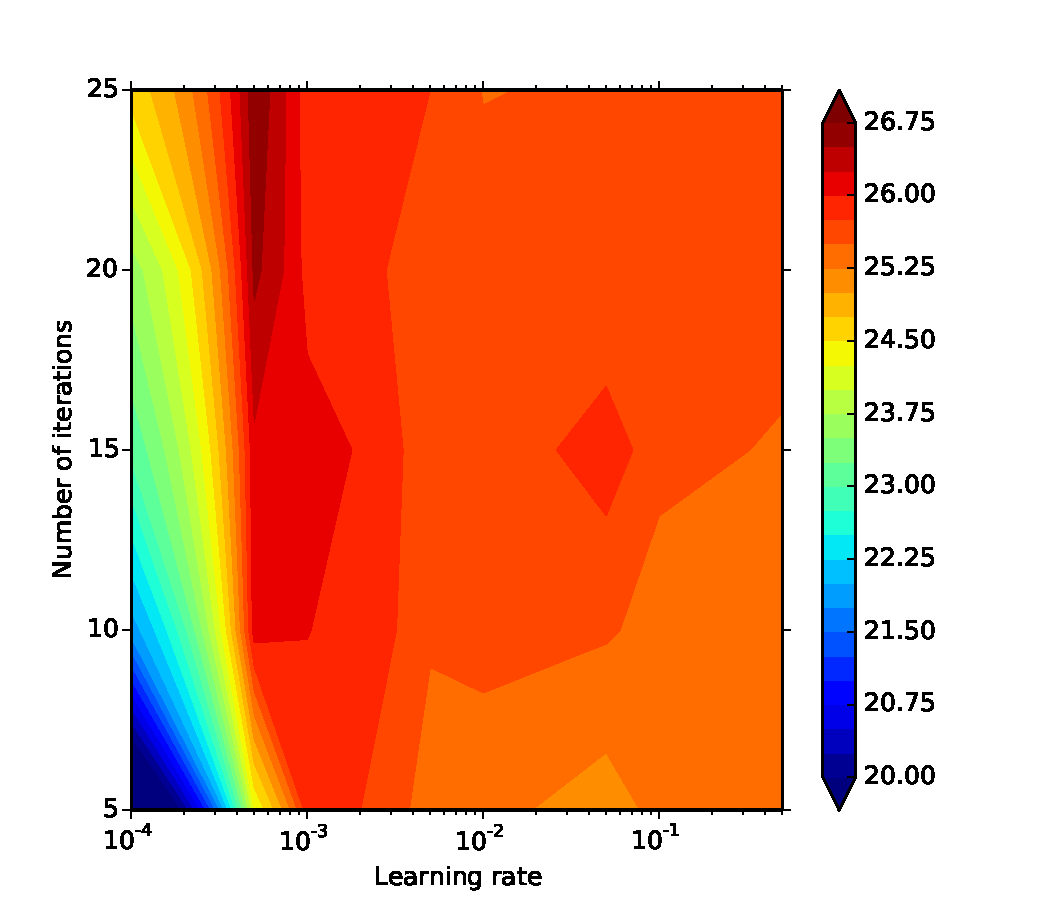
\includegraphics[width=\linewidth]{perceptron_gridsearch}
  	\caption{Mean cross-validation accuracy as a function of parameters $\alpha$ and number of iterations}
  	\label{fig:perc-gridsearch}
\end{figure}

After training our perceptron on the complete training set using these parameters, we submitted our results to Kaggle and obtained a test accuracy of 27.420\%. As an approximation of the test confusion matrix, we provide the confusion matrix for the combined validation sets in Figure \ref{fig:perc-confusion}. Note the perceptron's greater ability to identify 0s and 1s compared to other digits.
\begin{figure}[h!]
	\centering
	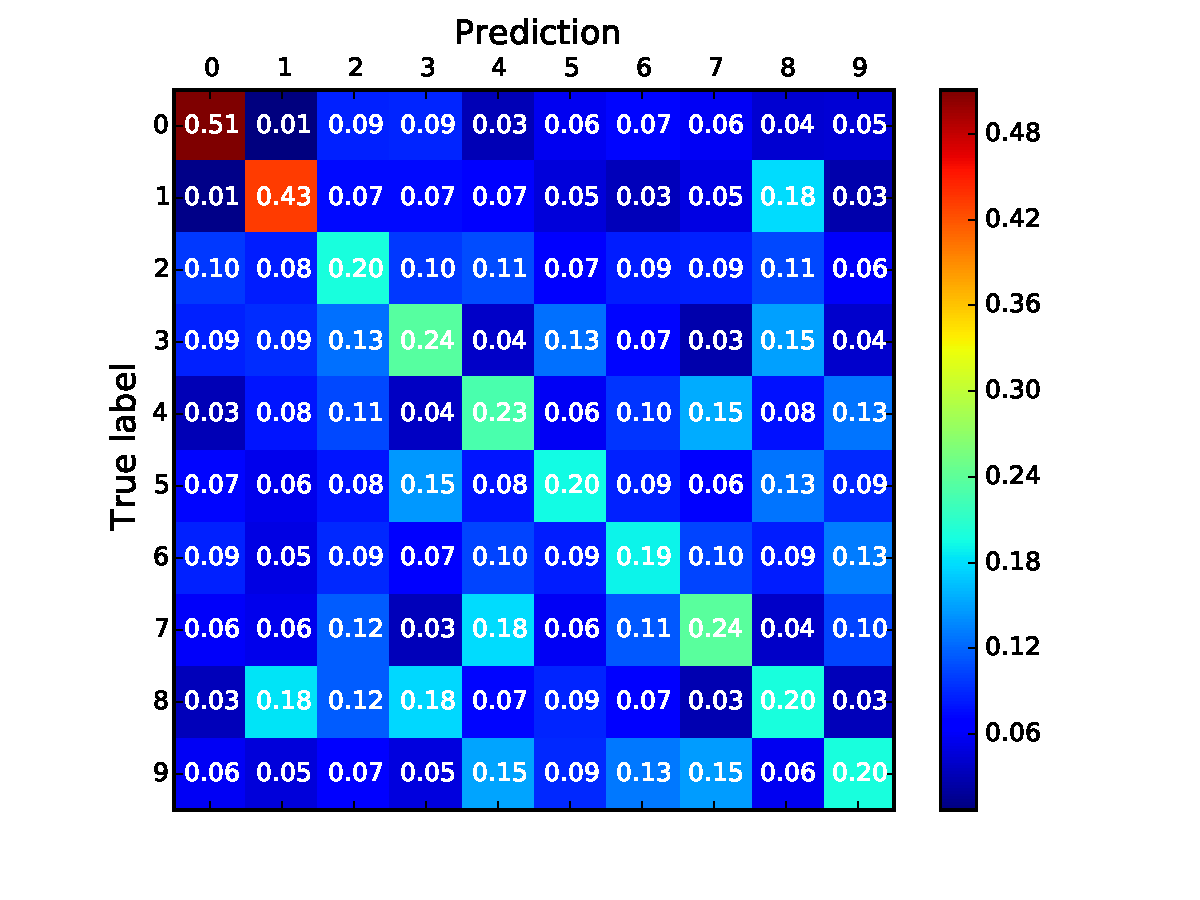
\includegraphics[width=\linewidth]{perceptron_confusion}
  	\caption{Validation confusion matrix for perceptron}
  	\label{fig:perc-confusion}
\end{figure}

\subsection{Neural Network}
Try a baseline net with the three feature sets, compare (5-fold cross-validation).

Use the best feature set to find best hyperparameters with cross-validation. You should probably try random search rather than gridsearch (faster and just as good or better), for some set number of configurations. Use some graph to show the hyperparameter space results. Plot validation confusion matrix. Say the test set (kaggle) result using best model found during crossval.

\subsection{Linear SVM}

\subsection{Convolutional Neural Network}
Only appropriate features = raw pixels. Applied contrast normalization on top of standardization.

Due to limited time, we can only sample a small sample of the hyperparameter space.

\section{Discussion}% pros/cons of approach & methodology (and alternatives)
Why is it better at classifying 0s and 1s? (Check number of examples in classes--could be Benford's law?

Using Gabor filters as a kernel rather than feature \cite{Sabri}

Other version of dropout \cite{Wan}

Pretraining \cite{Erhan}

Others: \cite{Rowley}, \cite{Simard}

{\bfseries We hereby state that all the work presented in this report is that of the authors.}

\bibliographystyle{abbrv}
\bibliography{references}

\appendix
\label{appendix}

\section{Additional results}
\label{sec:additional-results}

\begin{figure}[h!]
	\centering
	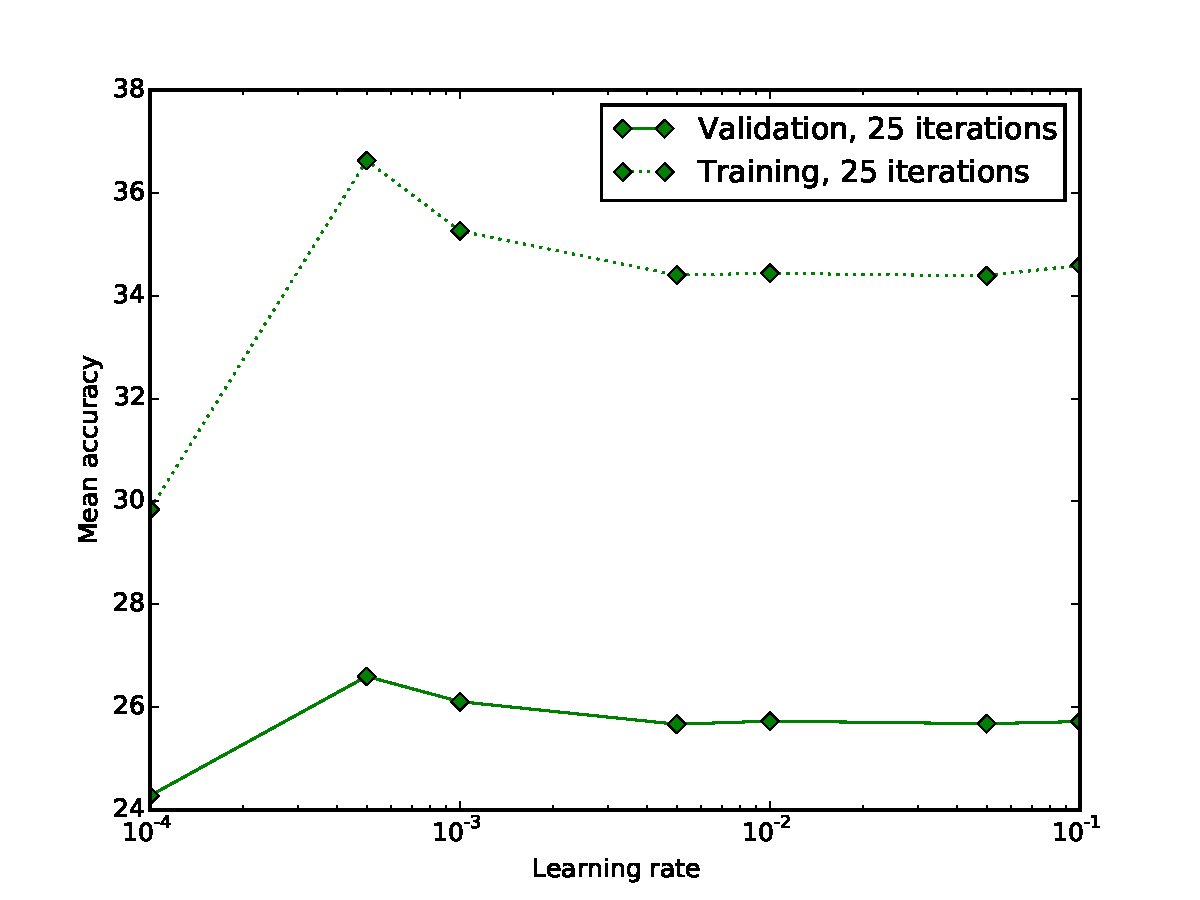
\includegraphics[width=\linewidth]{perceptron_learningrate}
  	\caption{Cross-validation over $\alpha$ with perceptron, keeping \# iterations optimal}
  	\label{fig:perc-learningrate}
\end{figure}
\begin{figure}[h!]
	\centering
	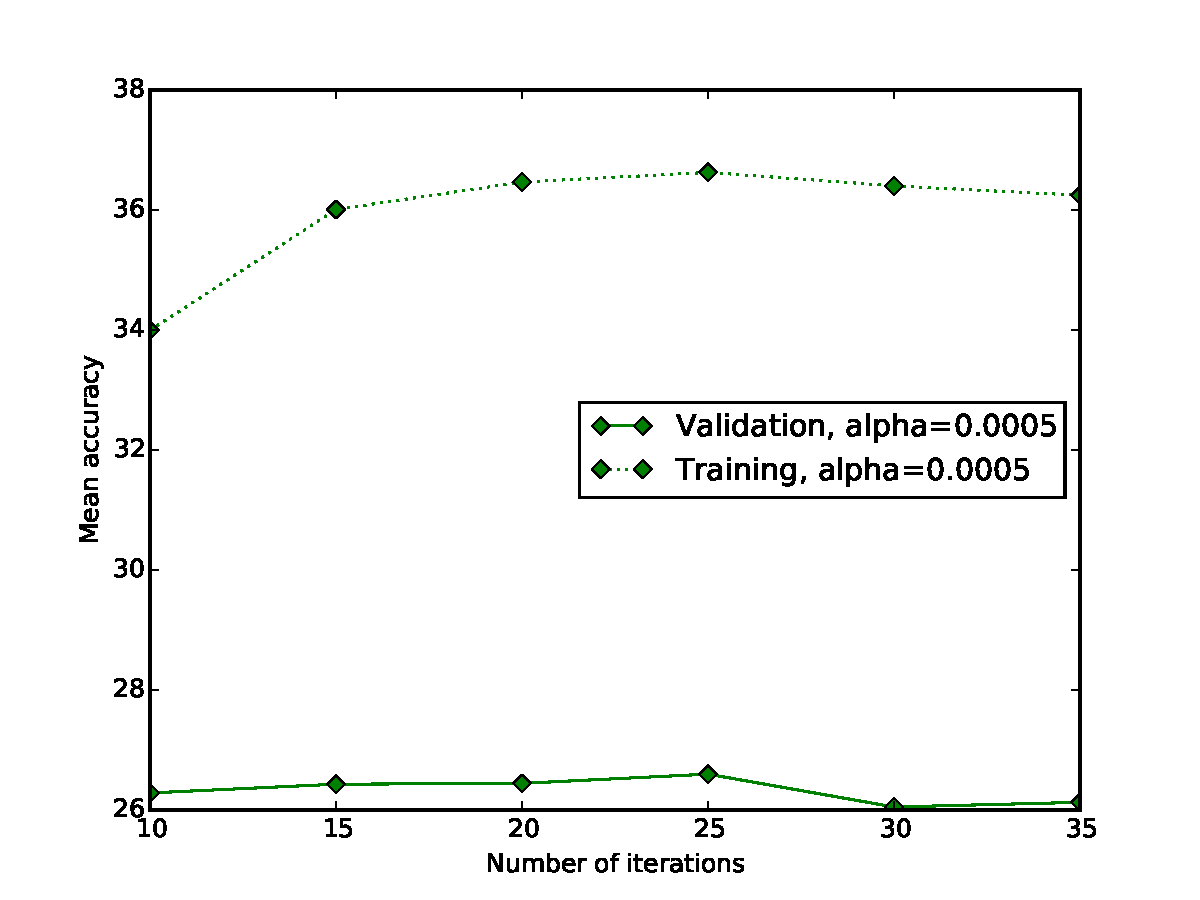
\includegraphics[width=\linewidth]{perceptron_iterations}
  	\caption{Cross-validation over \# of iterations with perceptron, keeping $\alpha$ optimal}
  	\label{fig:perc-iterations}
\end{figure}


\balancecolumns
\end{document}